\documentclass{article}



\usepackage[utf8]{inputenc}

% \usepackage{natbib}
\usepackage{hyperref}

\usepackage{graphicx}

% \usepackage[colorinlistoftodos]{todonotes}

\usepackage{parskip}
\setlength{\parskip}{10pt}

\usepackage{tikz}
\usetikzlibrary{arrows, decorations.markings}

% \usepackage{tikz-dependency}
% \usepackage{svg}

\usepackage{chngcntr}
\counterwithout{figure}{section}


\begin{document}


\begin{titlepage}


\centering


{\scshape\LARGE Master thesis project planning report\\}

\vspace{0.5cm}

{\huge\bfseries Efficient conversion from Dependency Trees to Abstract Syntax Trees in Natural Language Processing\\}

\vspace{2cm}

{\Large Andreas Källberg anka.213@gmail.com\\}

\vspace{1.0cm}

{\large Supervisor at CSE: Aarne Ranta\\}

\vspace{1.5cm}

{\large Relevant completed courses student 1:\par}

% {\itshape List (course code, name of course)\\}
{\itshape
    TIN092 Algorithms\\
    TDA342 Advanced functional programming\\
    DAT151 Programming language technology
\\}


    % \item DAT350 Types for programs and proofs

\vfill



\vfill

{\large \today\\}


\end{titlepage}


% The planning report is due 2 or 4 weeks after the start of you thesis project (date of registration in ladok). The planning report has to be approved by your examiner and should be developed in close collaboration with your supervisor. The planning report should be a development of the thesis proposal. The following points are a good start:

% Preliminary title.
% Background to the assignment. Why is it relevant?
% Aim for the work. What should be accomplished?
% The formulation of the problem at hand and, the assignment. This should include an extended version of the scientific problem definition and references to knowledge within the area given in the thesis proposal.
% Limitations. What should be left out and why?
% Method of accomplishment. How should the work be carried out?
% Risk analysis and ethical considerations.
% Time plan.

% The time plan should give an approximate date when the work is to be finished. It should also list mandatory seminars and milestones for the project with dates for critical steps that are needed to finish the work (which can include, depending on programme, e.g., intermediate report, mandatory seminars, presentation, opposition, and final report).


% 1. Intro
% - dep trees,
%  UD
%  - abstr trees, GF
%  - strengths and weaknesses
%   -> useful synthesis: UD-GF
%   -> applications:
%     - translation  - CL 2020
%     - semantics    - CL 2020
%     - concept alignment - Arianna
%     - SMU work - analysis of real world law text

\section{Introduction}
Something general about rule based NLG and NLP
and computer grammars

\subsection{Dependency trees and Universal Dependencies}
Dependency trees is a way of doing things

Universal Dependencies is a specifc dep tree thing for NLG

% Universal Dependencies\cite{mcdonald-al-2013} (UD) is another grammar formalism which uses machine-learning for parsing, which allows it to use context more in order to guess which interpretation was intended. The training data is based on a large set of sentences, which have been manually tagged with labels and a tree structure.

\subsection{Abstract trees and Grammatical Framework}

Grammatical Framework\cite{ranta-2004} (GF) is a formalism for describing natural language grammars as code, which allows converting between natural language and a language-independent abstract syntax. It is split into a generic resource grammar that covers morphology and the language as a whole and application grammars for a more narrow domain which allows a more semantic abstract syntax. When you try to write a grammar that covers a very wide domain, you will often get an over-generating grammar where each sentence can be parsed in very many ways into many different trees, where usually only one is the intended way.

\subsection{Strengths and weaknesses}

% % Grammatical Framework has [some] advantages for [usecase], so it would be useful to be able to parse using UD and then get out a GF tree. A
While the machine-learning based approach of UD allows it to guess the correct tree better for ambiguous sentences and allows it to handle grammatically incorrect sentences better, GF is much more capable when
it comes to performing transformations on the sentences, while maintaining correct morphology and grammar. This makes it attractive to parse sentences
using UD and then convert the parsed trees to GF trees in order to perform further transformations.

% There exists a proof-of-concept implementation of a tool for converting between the trees for GF and UD,
% with the help of so called labels files which describe the mapping between UD labels and GF functions,
% called gf-ud, which contains both a component for converting from UD to GF, called ud2gf\cite{kolachina-ranta-2017}
% and a component for converting from GF to UD, called gf2ud\cite{kolachina-ranta-2016}. This work will focus on the ud2gf component.

% The labels files can also contain macros, which allows constructing virtual GF functions during the translation from UD, which will be expanded to real GF functions at the end of the translation.
% These can, among other uses, be used to preserve information from the UD labels about subtrees, which can then be used at later points of the transformation to ensure that the desired GF tree is produced.

% % Maybe mention the macros in the labels files

% % There exists naive implementation based on a brute-force algorithm \cite{kolachina-ranta-2017}

% % Briefly describe and motivate the project, and convince the reader of the importance of the proposed thesis work.
% % A good introduction will answer these questions: Why is addressing these challenges significant for gaining new knowledge
% % in the studied domain? How and where can this new knowledge be applied?


% Background to the assignment. Why is it relevant?
% The formulation of the problem at hand and, the assignment. This should include an extended version of the scientific problem definition and references to knowledge within the area given in the thesis proposal.
\section{Background and Problem}

% 2. Background & Problem
% - old ud-gf
% - newer naive approach - github + article 2017
%   - limitations
%   - performance

% The current ud2gf implementation has some limitations. It quickly becomes extremely slow for sentences more than a couple of words and/or
% when using large GF-grammars, e.g. ones containing Wordnet\cite{angelov2016predicting}. Additionally, if the structure differs too much between the representation of a sentence in UD format and as a GF tree, it is not possible to describe the required transformation in the current "labels file" language.

% For example, the adjectival phrase "cute, fluffy and furry"
% would be described in UD format as in Figures \ref{fig:ud_cute_text} and \ref{fig:ud_cute}.


% \begin{figure}
%     \begin{verbatim}
%     1  cute  cute  ADJ  JJ  Degree=Pos  0  root  _  FUN=cute_A
%     2  ,  ,  PUNCT  ,  _  3  punct  _  _
%     3  fluffy  fluffy  ADJ  JJ  Degree=Pos  1  conj  _  FUN=fluffy_A
%     4  and  and  CCONJ  CC  _  5  cc  _  FUN=and_Conj
%     5  furry  furry  ADJ  JJ  Degree=Pos  1  conj  _  FUN=furry_A
%     \end{verbatim}
%     % \begin{tabular}{|c|c|c|c|c|c|c|c|c|c|}
%     % \hline
%     % 1 & cute & cute & ADJ & JJ & Degree\=Pos & 0 & root & \_ & FUN\=cute\_A \
%     % \hline
%     % 2 & , & , & PUNCT & , & \_ & 3 & punct & \_ & \_ \
%     % \hline
%     % 3 & fluffy & fluffy & ADJ & JJ & Degree\=Pos & 1 & conj & _ & FUN\=fluffy\_A \
%     % \hline
%     % 4 & and & and & CCONJ & CC & \_ & 5 & cc & \_ & FUN\=and\_Conj \
%     % \hline
%     % 5 & furry & furry & ADJ & JJ & Degree\=Pos & 1 & conj & \_ & FUN\=furry\_A \
%     % \hline
%     % \end{tabular}
%     \caption{The phrase "cute, fluffy and furry" as a textual UD tree}
%     \label{fig:ud_cute_text}
% \end{figure}

% \begin{figure}
%     \centering
%     % \begin{dependency}
  \begin{deptext}[column sep=0.4cm]
      cute \& , \& fluffy \& and \& furry \\
    {\tt ADJ}\&{\tt PUNCT}\&{\tt ADJ}\&{\tt CCONJ}\&{\tt ADJ} \\
  \end{deptext}
  \depedge{2}{1}{punct}
  \depedge{0}{2}{conj}
  \depedge{4}{3}{cc}
  \depedge{0}{4}{conj}
\end{dependency} \\
%     % \includesvg{ud-annotatrix-corpus.svg}
%     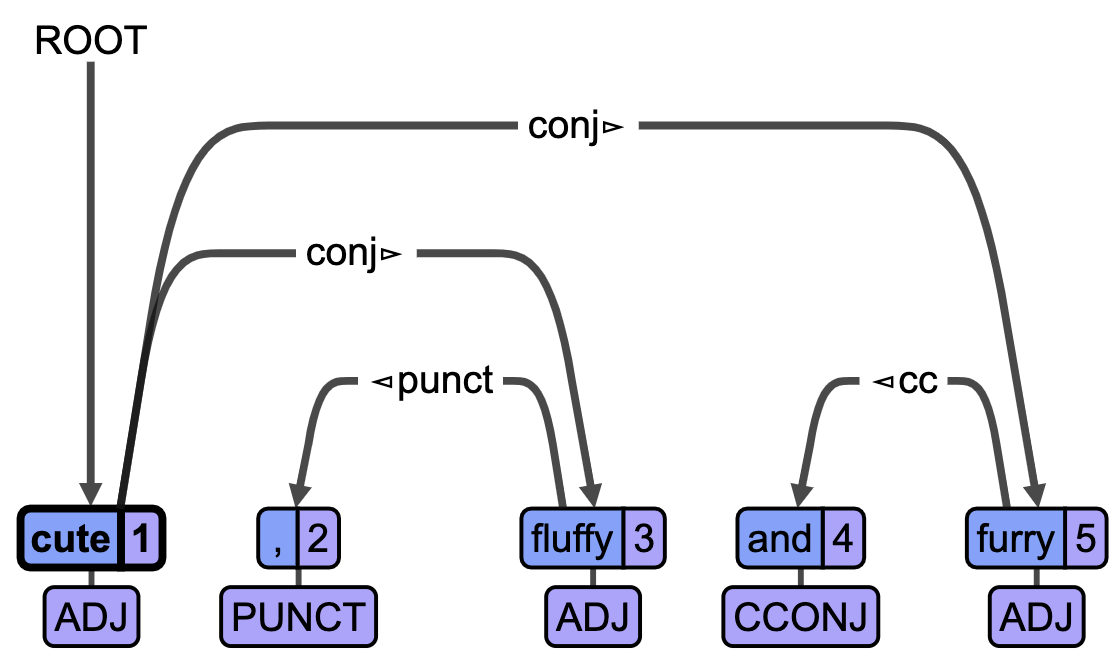
\includegraphics[width=0.7\textwidth]{ud_cute.png}
%     \caption{The phrase "cute, fluffy and furry" as a UD tree in graphical format}
%     \label{fig:ud_cute}
% \end{figure}
% % \include{}

% \begin{figure}
%     \centering
%     % \begin{dependency}
  \begin{deptext}[column sep=0.4cm]
      cute \& , \& fluffy \& and \& furry \\
    {\tt ADJ}\&{\tt PUNCT}\&{\tt ADJ}\&{\tt CCONJ}\&{\tt ADJ} \\
  \end{deptext}
  \depedge{2}{1}{punct}
  \depedge{0}{2}{conj}
  \depedge{4}{3}{cc}
  \depedge{0}{4}{conj}
\end{dependency} \\
%     % \includesvg{ud-annotatrix-corpus.svg}
%     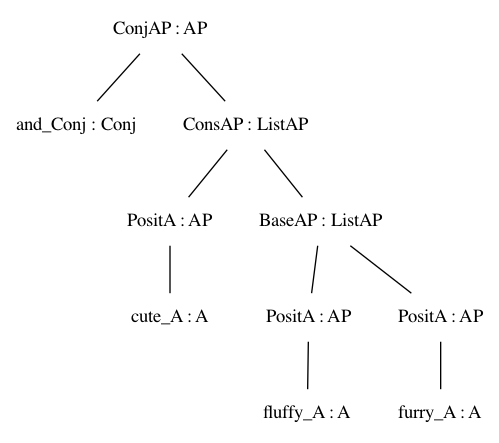
\includegraphics[width=0.7\textwidth]{cute_gf.png}
%     \caption{The phrase "cute, fluffy and furry" as a GF tree in graphical format. }
%     \label{fig:gf_cute}
% \end{figure}

% while the GF version of the same tree, shown in Figure \ref{fig:gf_cute}, would look like this:

% \begin{verbatim}
% ConjAP and_Conj (ConsAP (PositA cute_A)
%                         (BaseAP (PositA fluffy_A) (PositA furry_A)))
% \end{verbatim}
% Here we can see that in UD, the word "cute" is in the root, while the conjunction "and" is at the bottom of the tree, while in GF the conjunction is a direct child of the root. This transformation can not be preformed by the simple single-layer transformations that are available in the current macro-system for labels files.

% % Ideas:
% %
% % - Limits on how to transform trees - solution: extend language. currently hack using lambda calculus, but maybe better macros
% %
% % - Evaluate effectiveness of tool
% %
% % - (somewhere mention the performance boosts and analyse the complexity of it)

% % This section is optional. It may be used if there is a need to describe the problem that you want to solve in more technical
% % detail and if this problem description is too extensive to fit in the introduction.

% % From elsewhere:
% % - Background: GF \cite{ranta-2004}, UD \cite{nivre-etal-2016-universal},
% %   - previous work: gf2ud \cite{kolachina-ranta-2016}, ud2gf \cite{kolachina-ranta-2017}
% % - Describe the new algorithm
% % - Extending the macro language
% %   - Need for improvement: to match "fluffy and cute" needs 2 levels of nesting
% %   - Solution: continuations
% % - Case study: legal language

% The translation described by a labels file is not one-to-one and there are often many possible GF trees that a UD tree could be translated to. The possible trees are currently ranked by completeness, as in how many of the words are included in the generated tree. However this ranking is incomplete and in case two possible trees, with the same GF category, cover the same words, an arbitrary tree will be chosen. A better choice could be to also check the linearization of these trees and rank those whose linearization is more similar to the original string higher. It would also be possible to completely exclude trees with differing linearization, but that would run counter to the goal of robustness.

% Another problem is that it can sometimes be difficult to debug why a rule in a labels file is not firing, so it would be useful to have a debugging tool to help diagnosing such issues.


% 3. The new algorithm
% - definitions
% - examples
% - how annotations work

% 4. Evaluation
% - synthetic experiment: RGL -> UD -> RGL
%   - completeness - kan alltid få ett fullständigt träd
%   - accuracy
%   - performance
%   - error analysis

\section{Context}

% This work is mostly a continuation of the work in \cite{kolachina-ranta-2017}.

% A practical problem for which this tool can be useful can be found in \cite{listenmaa-etal-2021-towards}. In the Future Work section, under "Robust fall-back options", gf2ud is mentioned as a possible solution to making the parser more robust.

% % Use one or two relevant and high quality references for providing evidence from the literature that the proposed study indeed
% % includes scientific and engineering challenges, or is related to existing ones. Convince the reader that the problem addressed
% % in this thesis has not been solved prior to this project.


% Aim for the work. What should be accomplished?
\section{Goals and Challenges}

% 1. Analyze algorithms and improve performance. The main challenge here is to find an algorithm for finding matching trees without exponential complexity on the number of children of a node in the UD tree.

% 2. Improve flexibility of macro language, allowing changing the structure of the trees while translating from GF to UD. One challenge here is in figuring out either how to change the algorithms to support these more advanced transformations or to find a way to allow them without needing to change the algorithms.

% 3. Write a debugging tool, which analyzes exactly what it is that prevents a rule in a labels file from firing or what prevents that tree from being selected.
% One challenge here is how to explain to the user the issue for all the possible things that can go wrong.
% There is also an engineering challenge in making an algorithm that figures out what went wrong and why.
% % either repeating the steps of the algorithm in order to find the issues or transforming the algorithm in a way that they can explain what went wrong

% 4. If there is time, update the algorithm to look at the linearization in order to try to select trees that match the original string as closely as possible and evaluate what difference this makes. This is only possible with improved performance from goal 1, but keeping it fast will still be a challenge. There are also some challenges here in how it should interact with the advanced macros in goal 2. We also need to handle when a GF tree has multiple linearizations, e.g. if it results in a conjugation table.

% % improve

% % Analyse the complexity of old and new algorithm, evaluate effectiveness of ...

% % Describe your contribution with respect to concepts, theory and technical goals. Ensure that the scientific and engineering
% % challenges stand out so that the reader can easily recognize that you are planning to solve an advanced problem.

% Limitations. What should be left out and why?
\section{Limitations}

- Only the direction of ud2gf is studied here. why?
- other limitations?


\section{Approach}
% Method of accomplishment. How should the work be carried out?

% \subsection{Performance}

% 1. Finding the main source of slowness, which was done with profiling.

% 2. Analysing the current algorithms, which are based on brute-force, trying all combinations, with some simple filtering.

% 3. Finding a better algorithm, which avoids exploring paths that could never be the correct answer and which avoids duplicate work.

% 4. Analysing algorithmic complexity of both algorithms and testing the practical performance to confirm the results.

% \subsection{Flexibility}

% In order to allow changing the shape of trees when translating from UD to GF, the macro language needs to be expanded.
% A first prototype of this
% can be done with minimal code changes by making macro expansion recursive and then representing the code for the transformation in Church-encoding, inspired by lambda-calculus.

% This approach can be evaluated by seeing how well it covers different tree shape changes for different trees one would encounter.

% It could also be worthwhile to make a more user-friendly version of the advanced macros that can be understood without knowing about Church-encoding

% \subsection{Debugging tool}
% Go through each component of the algorithms in order to find where applying a rule can go wrong and add detection for them. Additionally try out the debugging tool on a real grammar, e.g. in the context of \cite{listenmaa-etal-2021-towards}, in order to find edge-cases which were not handled by the debugging tool.

% % Trial and error, whenever a problem arises that the tool doesn't find a helpful explanation for, try to add support for it.

% \subsection{Linearization-aware translation}
% Here we need a way to determine which linearization is actually closer and when to keep multiple options for a later stage of the translation. Some care also needs to be taken in determining which trees can be tossed away and which ones need to be kept around for a later stage.

% Evaluating if the results are better with this version can be done in a large part by comparing the input string with the resulting string after translating to GF and linearizing.

% % Various scientific approaches are appropriate for different challenges and project goals. Outline and justify the ones that
% % you have selected. For example, when your project considers systematic data collection, you need to explain how you will analyze
% % the data, in order to address your challenges and project goals.
% %
% % One scientific approach is to use formal models and rigorous
% % mathematical argumentation to address aspects like correctness and efficiency. If this is relevant, describe the related algorithmic
% % subjects, and how you plan to address the studied problem. For example, if your plan is to study the problem from a computability aspect,
% % address the relevant issues, such as algorithm and data structure design, complexity analysis, etc.  If you plan to develop and
% % evaluate a prototype, briefly describe your plans to design, implement, and evaluate your prototype by reviewing at most two relevant
% % issues, such as key functionalities and their evaluation criteria.
% %
% % The design and implementation should specify prototype properties,
% % such as functionalities and performance goals, e.g., scalability, memory, energy. Motivate key design selection, with respect to state
% % of the art and existing platforms, libraries, etc.
% %
% % When discussing evaluation criteria, describe the testing environment, e.g., test-bed
% % experiments, simulation, and user studies, which you plan to use when assessing your prototype. Specify key tools, and preliminary
% % test-case scenarios. Explain how and why you plan to use the evaluation criteria in order to demonstrate the functionalities and
% % design goals. Explain how you plan to compare your prototype to the state of the art using the proposed test-case evaluation scenarios
% % and benchmarks.


% Risk analysis and ethical considerations.
\section{Risk analysis and ethical considerations}
There are very little risks to speak of as the work is

There are no ethical considerations to speak of, since ...

(possibly evaluation data for the project and training data for the UD models)

% Time plan.
\section{Time plan}
Most of the practical work has already been completed by the authors of this thesis prior to the official start of this thesis.
The main parts that remain is evaluation and writing the report itself. Optionally, if there is time, some additional work to further improve the results can be performed (which ones?).

The plan is to complete the thesis before the summer of 2023.

Todo: more detailed plan

\section{References}



\bibliographystyle{plain}

\bibliography{main}




\end{document}
